\documentclass[a4paper,11pt,oneside]{article}

% $Id: ba-sample.tex 952 2006-03-06 20:14:35Z schoenw $

% To use this template, you have to have a halfway complete LaTeX
% installation and you have to run pdflatex, followed by bibtex,
% following by one-two more pdflatex runs.
%
% Note thad usimg a spel chequer (e.g. ispell, aspell) is generolz
% a very guud ideo.

\usepackage{times}		%% native times roman fonts
\usepackage{parskip}		%% blank lines between paragraphs, no indent
\usepackage[pdftex]{graphicx}	%% include graphics, preferrably pdf
\usepackage{amsmath}
\usepackage[pdftex]{hyperref}	%% many PDF options can be set here
\usepackage{amsthm,amssymb}
\usepackage{algorithm}
\usepackage{mathtools}
\usepackage{algpseudocode}
\usepackage[english]{babel}
\usepackage[utf8]{inputenc}
\pdfadjustspacing=1		%% force LaTeX-like character spacing

\hypersetup{
  pdfauthor = {Jos\'e Leal Domingues Neto 2},
  pdftitle = {List 1 - Data Mining},
  pdfkeywords = {datamining}
}

\begin{document}
  \thispagestyle{empty}
  \begin{flushleft}
    \textbf{\huge UFMG - DCC}\\
    \vspace*{6mm}
    \textbf{\huge List 1 - Data mining}
  \end{flushleft}
  \vspace*{6mm}
  \begin{flushleft}
    \textbf{\large Jos\'e Leal Domingues Neto}\\
    \href{mailto:dominguesn@gmail.com}{dominguesn@gmail.com} \\[2ex]
  \end{flushleft}
  \vspace*{1mm}
  \begin{flushleft}
    \textit{
      Data: \today \\
      Data mining}
  \end{flushleft}
  \vspace*{2mm}
\newpage


\section*{Algorithms and code}
All the code produced and used to achieve these answers are freely available in \href{https://github.com/jolealdoneto/datamining-list1}{https://github.com/jolealdoneto/datamining-list1}. This pdf simply gathers results.


\section*{Chapter 10, Q2}
\subsection*{a)} 
  Max:  ['ACT', 'AGTC', 'ATC', 'CAG', 'CGC', 'CTC', 'GAG', 'GCA', 'GCG', 'GTC', 'TCA', 'TCG']
\subsection*{b)} 
  Closed:  ['A', 'C', 'G', 'T', 'AT', 'ACT', 'AGC', 'AGT', 'ATC', 'CAG', 'CGC', 'CTC', 'GAG', 'GCA', 'GCG', 'GTC', 'AGTC']
\subsection*{c)} 
\begin{tabular}{l c}
Sequence & Support\\
\hline
AG & 5\\
G & 11\\
CA & 5\\
TC & 5\\
\end{tabular}
\subsection*{d)}
Result of spade formation: (Keys in dict is the sequence index) \\
AC 6 \{0: [2, 5, 7], 2: [3, 6], 3: [5], 4: [3], 5: [6, 8], 6: [4]\} \\
AG 6 \{0: [3, 8], 2: [5], 3: [3], 4: [2], 5: [5], 6: [2, 6]\} \\
AT 6 \{0: [4], 2: [4], 3: [4], 4: [4], 5: [7], 6: [3]\} \\
ACT 4 \{0: [4], 2: [4], 4: [4], 5: [7]\} \\
AGC 6 \{0: [5, 7], 2: [6], 3: [5], 4: [3], 5: [6, 8], 6: [4]\} \\
AGT 5 \{0: [4], 3: [4], 4: [4], 5: [7], 6: [3]\} \\
AGTC 4 \{0: [5, 7], 3: [5], 5: [8], 6: [4]\} \\
ATC 5 \{0: [5, 7], 2: [6], 3: [5], 5: [8], 6: [4]\} \\
CA 6 \{0: [6], 1: [4], 2: [7], 3: [2], 5: [4], 6: [5]\} \\
CC 4 \{0: [5, 7], 2: [6], 3: [5], 5: [6, 8]\} \\
CG 6 \{0: [3, 8], 1: [3], 2: [5], 3: [3], 5: [5], 6: [6]\} \\
CT 5 \{0: [4], 2: [4], 3: [4], 4: [4], 5: [7]\} \\
CAG 4 \{0: [8], 3: [3], 5: [5], 6: [6]\} \\
CGC 4 \{0: [5, 7], 2: [6], 3: [5], 5: [6, 8]\} \\
CTC 4 \{0: [5, 7], 2: [6], 3: [5], 5: [8]\} \\
GA 5 \{0: [6], 1: [4], 2: [2, 7], 5: [4], 6: [5]\} \\
GC 6 \{0: [5, 7], 2: [3, 6], 3: [5], 4: [3], 5: [3, 6, 8], 6: [4]\} \\
GG 4 \{0: [8], 2: [5], 5: [5], 6: [6]\} \\
GT 6 \{0: [4], 2: [4], 3: [4], 4: [4], 5: [7], 6: [3]\} \\
GAG 4 \{0: [8], 2: [5], 5: [5], 6: [6]\} \\
GCA 4 \{0: [6], 2: [7], 5: [4], 6: [5]\} \\
GCG 4 \{0: [8], 2: [5], 5: [5], 6: [6]\} \\
GTC 5 \{0: [5, 7], 2: [6], 3: [5], 5: [8], 6: [4]\} \\
TA 5 \{0: [6], 1: [4], 2: [7], 5: [4], 6: [5]\} \\
TC 6 \{0: [5, 7], 1: [2], 2: [6], 3: [5], 5: [3, 6, 8], 6: [4]\} \\
TG 5 \{0: [8], 1: [3], 2: [5], 5: [2, 5], 6: [6]\} \\
TCA 5 \{0: [6], 1: [4], 2: [7], 5: [4], 6: [5]\} \\
TCG 4 \{0: [8], 1: [3], 5: [5], 6: [6]\} \\

\subsection*{e)}
On paper

\section*{Chapter 12, Q5}
\subsection*{a)}
Variance = 70100502.5126

\begin{figure}[h]
  \caption{Histogram}
  \centering
    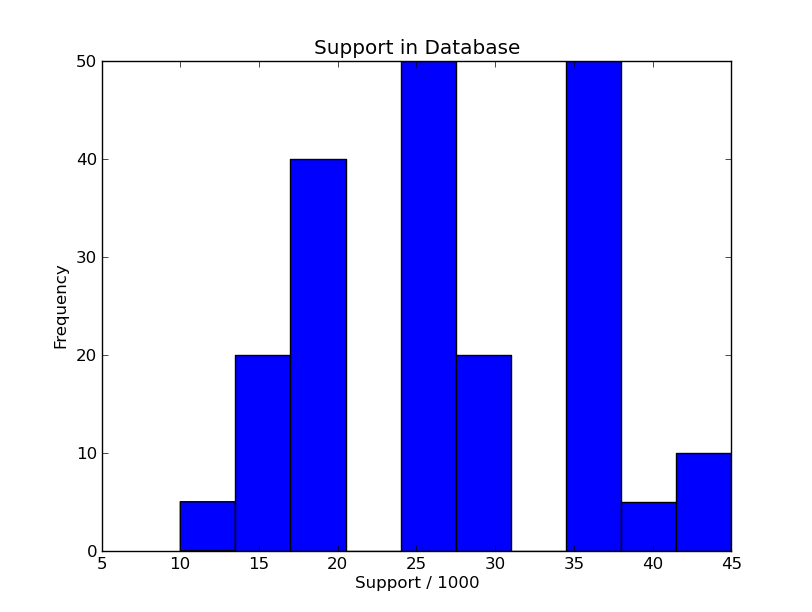
\includegraphics[width=0.8\textwidth]{cap12q5_a.png}
\end{figure}



\end{document}
